\newpage
\section{Implementierung}
Dieses Kapitel widmet sich der der konkreten Implementierung.

\subsection{\microphone}
Bevor eine Messung mit dem Board durchgeführt wird, ist zuerst ein Plausibilitätscheck durchgeführt worden. Dabei überprüft man, ob die beiden \microphone \platz Mikrofone korrekte Ergebnisse liefern. Der Aufbau ist durch das folgende Blockschaltbild \ref{img:blockschaltbild_plausibilitaetscheck} abgebildet. Abbildung \ref{img:picture_plausibilitaetscheck} zeigt den Aufbau im Laborraum.

\begin{figure}[H]
        \centering
        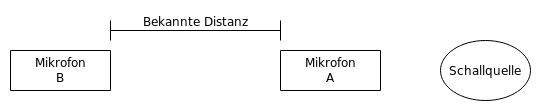
\includegraphics[width=0.9\textwidth]{images/plausibilitaetscheck.png}
        \caption{Versuchsaufbau als Blockschaltbild}
        \label{img:blockschaltbild_plausibilitaetscheck}
\end{figure}

\begin{figure}[H]
        \centering
        \hspace*{-1.9cm}
        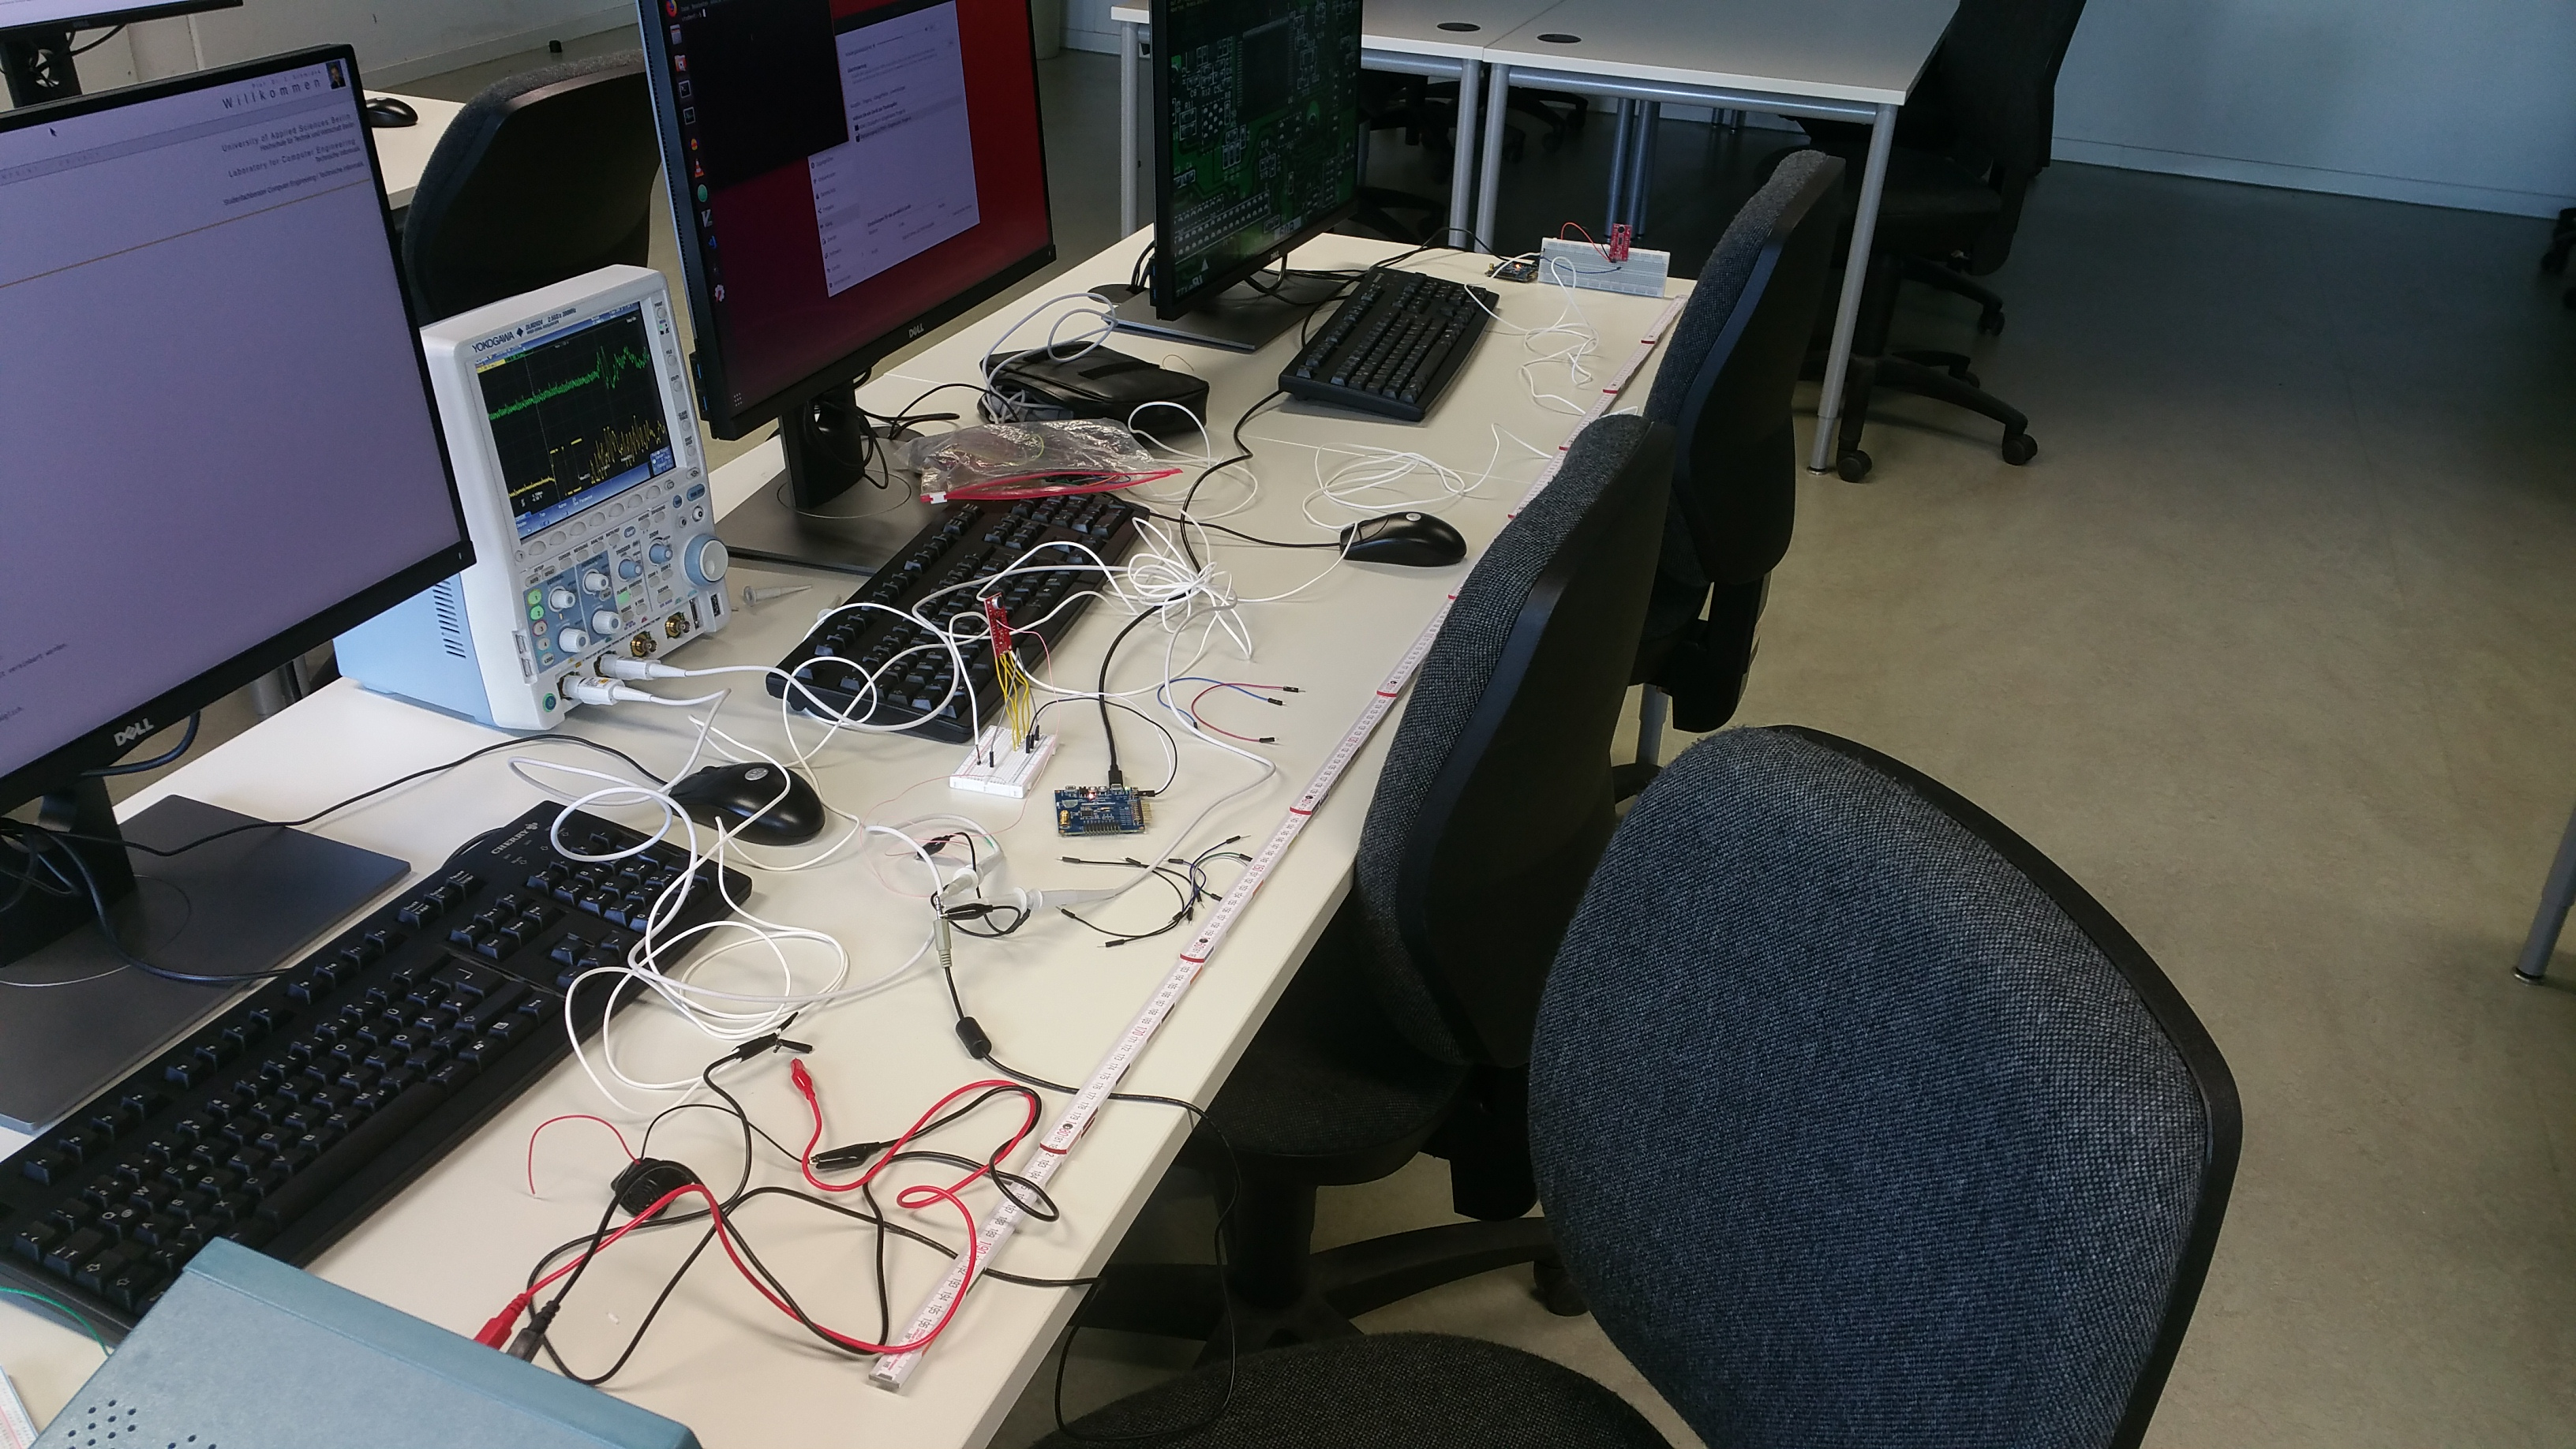
\includegraphics[width=1.2\textwidth]{images/plausibilitaetscheck_sparkfun_foto.jpg}
        \caption{Versuchsaufbau}
        \label{img:picture_plausibilitaetscheck}
\end{figure}

Die beiden Mikrofone sind an einem Oszilloskop angeschlossen. Es werden die \si{AUDIO}- und \si{GATE}-Ausgänge untersucht. Wenn die Schallquelle einen Ton aussendet (durch Klatschen oder ähnliches), passiert er zuerst das Mikrofon A und dann mit einer Verzögerung Mikrofon B. Mithilfe des bekannten Abstandes der beiden Mikrofone wird untersucht, ob das Ergebnis auf dem Oszilloskop mit dem Abstand der Mikrofone übereinstimmt. In Abbildung \ref{img:plausibilitaetscheck_oszi} sind vier verschiedene Signale abgebildet. Dabei entspricht Signal \textit{gelb} dem \si{GATE}-Ausgang von Mikrofon A und \textit{grün} dem \si{AUDIO}-Ausgang. Signal \textit{violett} und \textit{blau} entsprechen dem \si{GATE}- und \si{AUDIO}-Ausgang von dem zweiten Mikrofon.

\begin{figure}[H]
        \centering
        \hspace*{-1.9cm}
        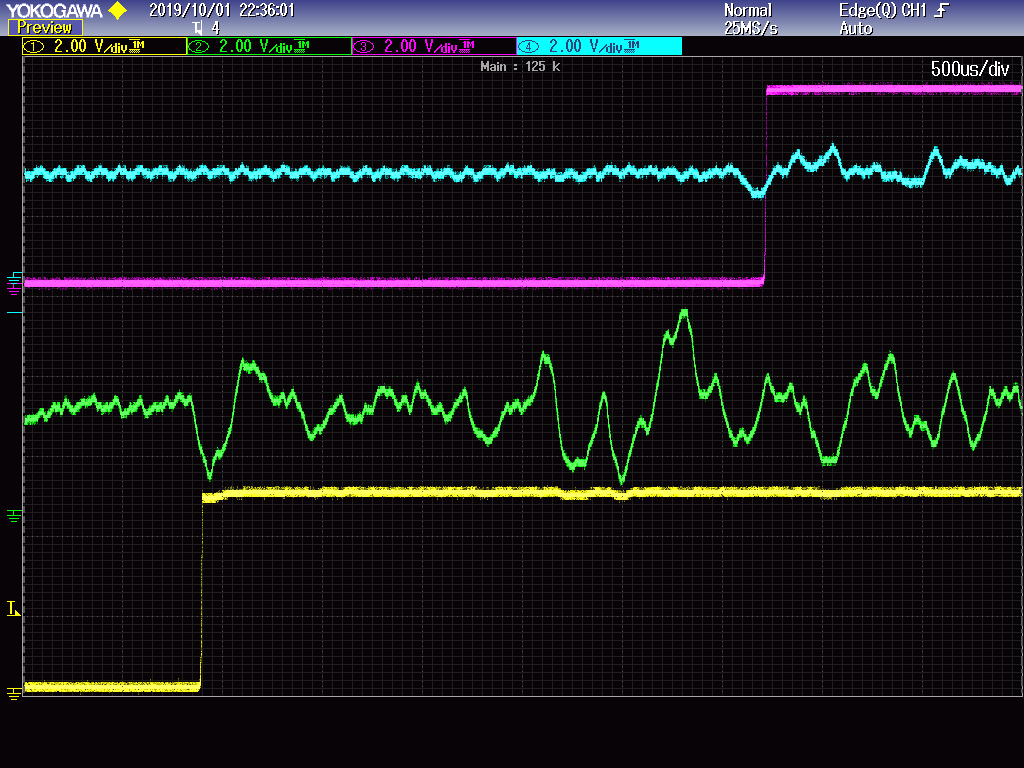
\includegraphics[width=1.2\textwidth]{images/plausibilitaetscheck_oszi.png}
        \caption{Verzögerung der Schallausbreitung}
        \label{img:plausibilitaetscheck_oszi}
\end{figure}

Es ist deutlich erkennbar, dass eine Verzögerung vorhanden ist. Die beiden \si{GATE}-Ausgänge liegen ungefähr \SI{2863}{\micro \second} auseinander. Mit einer Ausbreitungsgeschwindigkeit von \SI{0,034}{\centi\metre\per\micro\second} entspricht das ungefähr \SI{97,342}{\centi\metre}. Der gemessene Abstand ist \SI{100}{\centi\metre}. Diese Auswertung zeigt, dass die Verzögerung nur minimal von dem gemessenen Abstand abweicht. Es folgen weitere Messungen, bei dem anstatt eines Klatschen der verwendetete Tongeber verwendet wird. Dabei sitzt der Lautsprecher direkt neben einem der beiden Mikrofone. Das zweite Mikrofon sitzt \SI{1}{\metre}, \SI{2}{\metre} und \SI{3}{\metre} entfernt. Es folgen drei Tabellen (\ref{tab:plausibilitaetscheck_1m} - \ref{tab:plausibilitaetscheck_3m}) mit den Messwerten (Arithmetisches Mittel).

\begin{table}[H]
\centering
\caption{Messwerte bei \SI{1}{m} Entfernung}
\label{tab:plausibilitaetscheck_1m}
\begin{tabular}{|c|c|c|c|}
\hline
\multicolumn{4}{|c|}{\textbf{\SI{1}{m} Entfernung}}	\\ \hline
\textbf{Messwert von Mikrofon 1 [\si{\mu s}]} & \textbf{Messwert von Mikrofon 2 [\si{\mu s}]} & \textbf{Differenz [\si{\mu s}]} & \textbf{Distanz [\si{\centi\m}]}\\ \hline
595,00              & 4345,00             & 3750,00			& 127,50 	\\ \hline
603,00              & 4340,00             & 3737,00         & 125,05  	\\ \hline
461,00              & 4440,00             & 3979,00         & 135,28   	\\ \hline
608,00              & 4560,00             & 3952,00         & 134,36   	\\ \hline
641,00              & 4670,00             & 4029,00         & 136,98   	\\ \hline
443,00              & 4400,00             & 3957,00         & 134,53  	\\ \hline
450,00              & 4415,00             & 3965,00         & 134,81  	\\ \hline
634,00              & 4335,00             & 3701,00         & 125,83   	\\ \hline
638,00              & 4425,00             & 3787,00         & 128,75  	\\ \hline
640,00              & 4850,00             & 4210,00         & 143,14   	\\ \hline
\multicolumn{4}{|c|}{\textbf{Durchschnitt}}                    			\\ \hline
571,30              & 4036,50             & 3511,00         & 132,62	\\ \hline
\end{tabular}
\end{table}

\begin{table}[H]
\centering
\caption{Messwerte bei \SI{2}{m} Entfernung}
\label{tab:plausibilitaetscheck_2m}
\begin{tabular}{|c|c|c|c|}
\hline
\multicolumn{4}{|c|}{\textbf{\SI{2}{m} Entfernung}} \\ \hline
\textbf{Messwert von Mikrofon 1 [\si{\mu s}]} & \textbf{Messwert von Mikrofon 2 [\si{\mu s}]} & \textbf{Differenz [\si{\mu s}]} & \textbf{Distanz [\si{\centi\m}]}\\ \hline
476,00              & 20150,00            & 19674,00		& 668,91	\\ \hline
458,00              & 37900,00            & 37442,00        & 1273,02	\\ \hline
471,00              & 36150,00            & 35679,00        & 1213,08  	\\ \hline
681,00              & 38750,00            & 38079,00        & 1294,68  	\\ \hline
452,00              & 38150,00            & 37698,00        & 1281,73  	\\ \hline
466,00              & 34150,00            & 33684,00        & 1145,25	\\ \hline
675,00              & 38750,00            & 38075,00        & 1294,55  	\\ \hline
450,00              & 33550,00            & 33100,00        & 1125,40  	\\ \hline
447,00              & 32600,00            & 32153,00        & 1093,20  	\\ \hline
460,00              & 35800,00            & 35340,00        & 1201,56  	\\ \hline
\multicolumn{4}{|c|}{\textbf{Durchschnitt}}                   	 		\\ \hline
503,60              & 34595,00            & 34072,40        & 1159,13  	\\ \hline
\end{tabular}
\end{table}

\begin{table}[H]
\centering
\caption{Messwerte bei \SI{3}{m} Entfernung}
\label{tab:plausibilitaetscheck_3m}
\begin{tabular}{|c|c|c|c|}
\hline
\multicolumn{4}{|c|}{\textbf{\SI{3}{m} Entfernung}} \\ \hline
\textbf{Messwert von Mikrofon 1 [\si{\mu s}]} & \textbf{Messwert von Mikrofon 2 [\si{\mu s}]} & \textbf{Differenz [\si{\mu s}]} & \textbf{Distanz [\si{\centi\m}]}\\ \hline
454,00              & 33450,00            & 32996,00		& 1121,86	\\ \hline
428,50              & 35800,00            & 35371,50        & 1202,63   \\ \hline
474,00              & 37650,00            & 37176,00        & 1263,98   \\ \hline
429,00              & 33500,00            & 33071,00        & 1124,41  	\\ \hline
437,50              & 37700,00            & 37262,50        & 1266,92   \\ \hline
439,50              & 35550,00            & 35110,50		& 1193,75	\\ \hline
435,50              & 25200,00            & 24764,50        & 841,99	\\ \hline
437,50              & 23800,00            & 23362,50        & 794,32	\\ \hline
430,00              & 24950,00            & 24520,00        & 833,68	\\ \hline
427,50              & 25800,00            & 25372,50        & 862,66	\\ \hline
\multicolumn{4}{|c|}{\textbf{Durchschnitt}}                 			\\ \hline
439,30              & 31340,00            & 30900,70    	& \\ \hline
\end{tabular}
\end{table}

Aus den obigen Tabellen ist zu erkennen, dass Mikrofon \si{1} mindestens \SI{439,30}{\mu\s} braucht, um den Ton wahrzunehmen. Allerdings steht das Mikrofon \si{1} direkt neben dem Tongeber. Durch Latenzen beim Mikrofon ist dieser Messwert nicht null. Allerdings nimmt die Latenz mit der Entfernung ab, woraus keine konstante Abweichung entnommen werden kann. Weitherhin ist zu erkennen, dass es eine deutliche Abweichung gibt, obwohl der Versuch mit Klatschen als Tongeber ein brauchbares Ergebnis produzierte. Dieses Messergebnis zeigt, dass der Lautsprecher und das Mikrofon zusammen keine brauchbaren Messergebnisse erzielen, da die Abweichungen irregulär ansteigen.

\subsection{Modul A}
Das Modul A untersucht die Verzögerung des Masters vom Detektieren eines Mikrofons und des Aufrufs der Interruptroutine. Das Mikrofon liefert bei Erkennen eines Tons einen Pegelwechsel von \si{LOW} - \si{HIGH}. In der Interruptroutine des Masters wird ein Pin auf \si{HIGH} gesetzt. Dabei besitzt der Slave den Lautsprecher. Es wird ein \si{PIEP}-Ton erzeugt. Master und Slave agieren unabhängig voneinander. Das Oszilloskop wurde an dem \si{GATE}-Ausgang des Mikrofons angehängt und an dem Pin, der in der Interruptroutine auf \si{HIGH} gesetzt worden ist. Darüber hinaus ist die Schallquelle dreimal versetzt worden, um Abweichungen abhängig von der Distanz vornehmen zu können. Es folgt eine Tabelle (\ref{tab:modul_A}) mit den Messwerten. Die Messwerte wurden von dem Oszilloskop abgelesen.

\begin{table}[H]
\centering
\caption{ISR-Verzögerung Mikrofon-\board \platz bei unterschiedlicher Kabellänge}
\label{tab:modul_A}
\begin{tabular}{|c|c|c|}
\hline
\multicolumn{3}{|c|}{\textbf{Messwert [\si{\mu s}]}} \\ \hline
\textbf{\SI{1}{\m}}   & \textbf{\SI{2}{\m}}   & \textbf{\SI{3}{\m}}   \\ \hline
67,00          & 91,00          & 66,00          \\ \hline
78,00          & 83,00          & 88,50          \\ \hline
94,00          & 86,00          & 72,50          \\ \hline
81,50          & 59,00          & 75,50          \\ \hline
78,50          & 82,00          & 83,00          \\ \hline
87,50          & 76,00          & 82,50          \\ \hline
74,00          & 87,50          & 92,50          \\ \hline
87,00          & 80,00          & 84,50          \\ \hline
88,50          & 88,00          & 88,00          \\ \hline
81,50          & 70,50          & 64,50          \\ \hline
\multicolumn{3}{|c|}{\textbf{Durchschnitt}}      \\ \hline
74,45          & 81,30          & 79,75          \\ \hline
\end{tabular}
\end{table}

Die resultierenden Durchschnittswerte weichen nur minimal voneinander ab. Somit hat die Distanz zwischen der Schallquelle und dem Mikrofon keinen Einfluss auf die Interruptzeit. Da die Interruptzeit nur minimal abweicht, kann diese Verzögerung weggerechnet werden.

\subsection{Modul B}
Dieses Modul untersucht die Abweichungen vom Aussenden eines \si{HIGH}-Signals des Masters bis zum Durchschalten des Mosfets beim Slave. Der Slave nimmt das \si{HIGH}-Signal vom Master durch eine Interruptroutine entgegen und setzt den \si{GATE}-Pin des Mosfets sofort auf \si{HIGH}. Der Master ist per Kabel mit dem Slave verbunden. Auch hier wird die Kabellänge verändert. Für dieses Modul wird kein Lautsprecher und kein Mikrofon benötigt.
\\
Es wird angenommen, dass die Interruptzeit nicht von der Kabellänge zwischen Master und Slave abhängig ist. Die Messwerte für eine Kabellänge von \SI{5}{\m} und einer direkten Verbindung sind wie folgt:

\begin{table}[H]
\centering
\caption{Verzögerung der Slave-ISR bei unterschiedlicher Kabellänge}
\label{tab:modul_B}
\begin{tabular}{|c|l|}
\hline
\multicolumn{2}{|c|}{\textbf{Messwert [\si{\mu s}]}}     \\ \hline
\textbf{Direkte Verbindung}  & \textbf{\SI{5}{\m}} \\ \hline
78,10                        & 92,00        \\ \hline
70,80                        & 74,00        \\ \hline
68,30                        & 87,00        \\ \hline
78,10                        & 91,80        \\ \hline
74,70                        & 84,80        \\ \hline
97,20                        & 89,60        \\ \hline
81,20                        & 70,40        \\ \hline
94,60                        & 90,80        \\ \hline
94,50                        & 76,80        \\ \hline
88,80                        & 67,40        \\ \hline
\multicolumn{2}{|c|}{\textbf{Durchschnitt}} \\ \hline
82,46                        & 82,63        \\ \hline
\end{tabular}
\end{table}

Auch hier zeigt sich, das die Interruptzeit nicht von der Kabellänge abhängig ist. Weiterhin ist die Interruptzeit des Slaves nahezu konstant -- dadurch kann auch diese Verzögerung weggerechnet werden. 

\subsection{Modul C}
Hierbei soll die Anstiegszeit des N-Mosfet ermittelt werden. Die Anstoiegszeit liegt laut dem Datenblatt bei \SI{40}{\nano\s}. Das verwendete Oszilloskop schafft es nicht, die Angabe zu überprüfen, da die Zeitauflösung nicht genau genug ist. Die Anstiegszeit verursacht eine Abweichung von $\si{0,000034}[\si{\centi\m\per\nano\s}] \cdot \si{40} [\si{\nano\s}] = \si{0,00136} [\si{\centi\m}]$. Diese Abweichung ist zu gering, um Einfluss auf das Endergebnis auszuüben, da sie erst ab der dritten Nachkommastelle Einfluss ausübt. Aufgrund dessen wird diese Abweichung vernachlässigt.

\subsection{Modul D}
\label{sec:modul_D}
Dieses Modul untersucht die Abweichungen vom Lautsprecher und dem Mikrofon. Dabei wird die Zeit zwischen dem Lautsprecher und dem \si{GATE}-Signal des \microphone s \platz gemessen. Der Masterknoten wird nicht benötigt. Der Slaveknoten besitzt den Lautsprecher und den dazugehörigen Mosfet. Er schaltet den Lautsprecher für \SI{40000}{\mu\s} an. Theoretisch muss der errechnete Wert aus der Distanz und der Schallgeschwindigkeit den gemessenen Werten auf dem Oszilloskop entsprechen. Messungen werden mit den Distanzen \SI{1}{m}, \SI{2}{m} und \SI{3}{m} vorgenommen. Es folgen drei Tabellen (\ref{tab:modul_D_1} - \ref{tab:modul_D_3}) mit den Messwerten. 

\begin{table}[H]
\centering
\caption{Abweichung zwischen Mikrofon und Lautsprecher bei \SI{1}{m}}
\label{tab:modul_D_1}
\begin{tabular}{|c|c|c|c|}
\hline
\multicolumn{4}{|c|}{\textbf{\SI{1}{\m} Entfernung}}                                                                                                              \\ \hline
\textbf{Theorie [\si{ms}]} & \textbf{Messwert [\si{ms}]} & \multicolumn{1}{l|}{\textbf{Differenz [\si{ms}]}} & \multicolumn{1}{l|}{\textbf{Distanz [\si{cm}]}} \\ \hline
2,94                      & 5,14                       & 2,19                                             & 74,76                                          \\ \hline
2,94                      & 5,14                       & 2,19                                             & 74,76                                          \\ \hline
2,94                      & 4,87                       & 1,92                                             & 65,58                                          \\ \hline
2,94                      & 4,87                       & 1,92                                             & 65,58                                          \\ \hline
2,94                      & 5,15                       & 2,20                                             & 75,10                                          \\ \hline
2,94                      & 4,88                       & 1,93                                             & 65,92                                          \\ \hline
2,94                      & 4,87                       & 1,92                                             & 65,58                                          \\ \hline
2,94                      & 4,90                       & 1,95                                             & 66,60                                          \\ \hline
2,94                      & 4,89                       & 1,94                                             & 66,26                                          \\ \hline
2,94                      & 4,90                       & 1,95                                             & 66,60                                          \\ \hline
\multicolumn{4}{|c|}{\textbf{Durchschnitt}}                                                                                                                \\ \hline
2,94                      & 4,96                       & 2,01                                             & 68,67                                          \\ \hline
\end{tabular}
\end{table}


\begin{table}[H]
\centering
\caption{Abweichung zwischen Mikrofon und Lautsprecher bei \SI{2}{m}}
\label{tab:modul_D_2}
\begin{tabular}{|c|c|c|c|}
\hline
\multicolumn{4}{|c|}{\textbf{\SI{2}{\m} Entfernung}}                                                                                                              \\ \hline
\textbf{Theorie [\si{ms}]} & \textbf{Messwert [\si{ms}]} & \multicolumn{1}{l|}{\textbf{Differenz [\si{ms}]}} & \multicolumn{1}{l|}{\textbf{Distanz [\si{cm}]}} \\ \hline
5,88                      & 11,38                      & 5,49                                             & 186,92                                         \\ \hline
5,88                      & 11,08                      & 5,19                                             & 176,81                                         \\ \hline
5,88                      & 11,66                      & 5,77                                             & 196,44                                         \\ \hline
5,88                      & 11,72                      & 5,83                                             & 198,48                                         \\ \hline
5,88                      & 12,00                      & 6,11                                             & 208,00                                         \\ \hline
5,88                      & 11,12                      & 5,23                                             & 178,00                                         \\ \hline
5,88                      & 11,48                      & 5,59                                             & 190,32                                         \\ \hline
5,88                      & 11,14                      & 5,25                                             & 178,76                                         \\ \hline
5,88                      & 11,72                      & 5,83                                             & 198,48                                         \\ \hline
5,88                      & 11,44                      & 5,55                                             & 188,96                                         \\ \hline
\multicolumn{4}{|c|}{\textbf{Durchschnitt}}                                                                                                                \\ \hline
5,88                      & 11,47                      & 5,59                                             & 190,10                                         \\ \hline
\end{tabular}
\end{table}




\begin{table}[H]
\centering
\caption{Abweichung zwischen Mikrofon und Lautsprecher bei \SI{3}{m}}
\label{tab:modul_D_3}
\begin{tabular}{|c|c|c|c|}
\hline
\multicolumn{4}{|c|}{\textbf{\SI{3}{\m} Entfernung}}                                                                                                              \\ \hline
\textbf{Theorie [\si{ms}]} & \textbf{Messwert [\si{ms}]} & \multicolumn{1}{l|}{\textbf{Differenz [\si{ms}]}} & \multicolumn{1}{l|}{\textbf{Distanz [\si{cm}]}} \\ \hline
8,82                      & 23,95                      & 15,12                                            & 514,30                                         \\ \hline
8,82                      & 35,70                      & 36,87                                            & 913,80                                         \\ \hline
8,82                      & 31,75                      & 22,92                                            & 779,50                                         \\ \hline
8,82                      & 24,25                      & 15,42                                            & 524,50                                         \\ \hline
8,82                      & 30,75                      & 21,92                                            & 745,50                                         \\ \hline
8,82                      & 22,30                      & 13,47                                            & 458,20                                         \\ \hline
8,82                      & 22,30                      & 13,47                                            & 458,20                                         \\ \hline
8,82                      & 34,00                      & 25,17                                            & 856,00                                         \\ \hline
8,82                      & 23,60                      & 14,77                                            & 502,40                                         \\ \hline
8,82                      & 26,15                      & 17,32                                            & 589,10                                         \\ \hline
\multicolumn{4}{|c|}{\textbf{Durchschnitt}}                                                                                                                \\ \hline
8,82                      & 27,47                      & 18,65                                            & 634,15                                         \\ \hline
\end{tabular}
\end{table}

Aus den Messwerten geht hervor, dass mit steigender Distanz der Fehler größer wird. Der Fehler steigt nicht linear an. Da kein Muster erkennbar ist, kann diese Abweichung nicht verrechnet werden. Da bei den vorherigen Modulen ein konstanter Fehler zu erkennen war, und dieses Modul ihn nicht aufweist, muss die Abweichung des Endergebnisses zwischen dem Lautsprecher und dem Mikrofon liegen. Eine solche Abweichung macht die Positionsbestimmung im Zentimeterbereich unmöglich. Die Ergebnisse aus Modul A lassen sich bei diesen Messungen bestätigen. Dadurch verfestigt sich der Verdacht, dass der Fehler beim Mikrofon oder beim Lautsprecher und dem Raum dazwischen liegen muss. Eine Vermutung für diesen größer werdenden Fehler ist, dass der Schall durch die Gegenstände im Raum abgelenkt wird und deswegen später beim Mikrofon ankommt. Weiterhin kann vielleicht durch eine Änderung der Tonfrequenz ein genaueres Ergebnis mit weniger Fehlern produziert werden. 

\subsection{Systemzeit}
Das RIOT OS stellt die Funktion $getSystemTime()$ zur Verfügung. Als Rückgabewert wird ein \si{32 Bit unsigned int} zurückgegeben. Die Analyse soll verdeutlichen, wie lange ein Funktionsaufruf dauert, um die Systemzeit auszulesen. Dabei wird vor dem Aufruf ein GPIO-Pin gesetzt und anschließend wieder zurückgesetzt. Die Differenz entspricht dabei ungefähr dem Systemaufruf. Es folgt Tabelle \ref{table:modul_E1} mit den Messwerten.

\begin{table}[H]
\centering
\caption{Messwerte für die Funktion $getSystemTime()$}
\label{table:modul_E1}
\begin{tabular}{|c|}
\hline
\textbf{Messwert [\si{\mu s}]} \\ \hline
7,26                       \\ \hline
7,09                       \\ \hline
7,43                       \\ \hline
7,10                       \\ \hline
7,42                       \\ \hline
6,93                       \\ \hline
7,26                       \\ \hline
7,10                       \\ \hline
7,27                       \\ \hline
7,25                       \\ \hline
\textbf{Durchschnitt}      \\ \hline
7,21                       \\ \hline
\end{tabular}
\end{table}

Aus den Messwerten erkennt man deutlich, dass der Aufruf nahezu konstant ist. Auch diese Abweichung kann im Endergebnis ausgeglichen werden. Bei diesem Aufruf werden verschiedene Funktionen aufgerufen. Der Timer-Wert wird in Ticks zurückgegeben und danach in \si{\mu}-Sekunden umgewandelt. Dadurch, dass verschiedene Funktionen aufgerufen werden und eine Umwandlung gemacht wird, kommen die \SI{7,21}{\mu\s} zustande. Der Durchschnittswert ist ein Maximalwert des Aufrufes, denn der Durchschnittswert beinhaltet das Setzen und Löschen des GPIOs. Die Messwerte für das Setzen und Löschen des GPIO werden durch die folgende Tabelle verdeutlicht.

\begin{table}[H]
\centering
\caption{Messwerte für das Setzen und Löschen eines GPIO}
\label{table:modul_E2}
\begin{tabular}{|c|}
\hline
\textbf{Messwert [\si{ns}]} \\ \hline
418,00                     \\ \hline
417,50                     \\ \hline
417,50                     \\ \hline
416,50                     \\ \hline
417,00                     \\ \hline
417,00                     \\ \hline
417,00                     \\ \hline
417,50                     \\ \hline
417,50                     \\ \hline
417,50                     \\ \hline
\textbf{Durchschnitt}      \\ \hline
417,25                     \\ \hline
\end{tabular}
\end{table}

Aus dem Durchschnittswert ergibt sich eine Abweichung von $0,014178 \; cm$. Dieser ist zu gering, um auf die Messwerte der Funktion $getSystemTime()$ Einfluss zu nehmen. Somit können die Messwerte aus Tabelle \ref{table:modul_E2} ohne Fehler betrachtet werden.


\subsection{Zeitsynchronisation}
Bei den bisherigen Messungen war der Master mit Hilfe eines Kabels mit dem Slave verbunden. In der Endanwendung jedoch ist der Master drahtlos mit dem Slave verbunden. Bevor die Zeitsynchronisation in die Software eingefügt werden kann, wird geprüft, welche Genauigkeit die Zeitsynchronisation erreicht. Dabei baut man zwei \board \platz nebeneinander auf. Insgesamt werden hundert Zeitsynchronisation (PTP) nacheinander durchgeführt. Danach bereitet und wertet man die Ergebnisse graphisch auf und wertet sich aus. Es wird nur auf die Variable $t_{prop}$ (Propagation Delay) eingegangen, da diese die Laufzeitverzögerung zwischen Master und Slave entspricht.
 
\begin{figure}[H]
        \centering
        \hspace*{-1.7cm}
        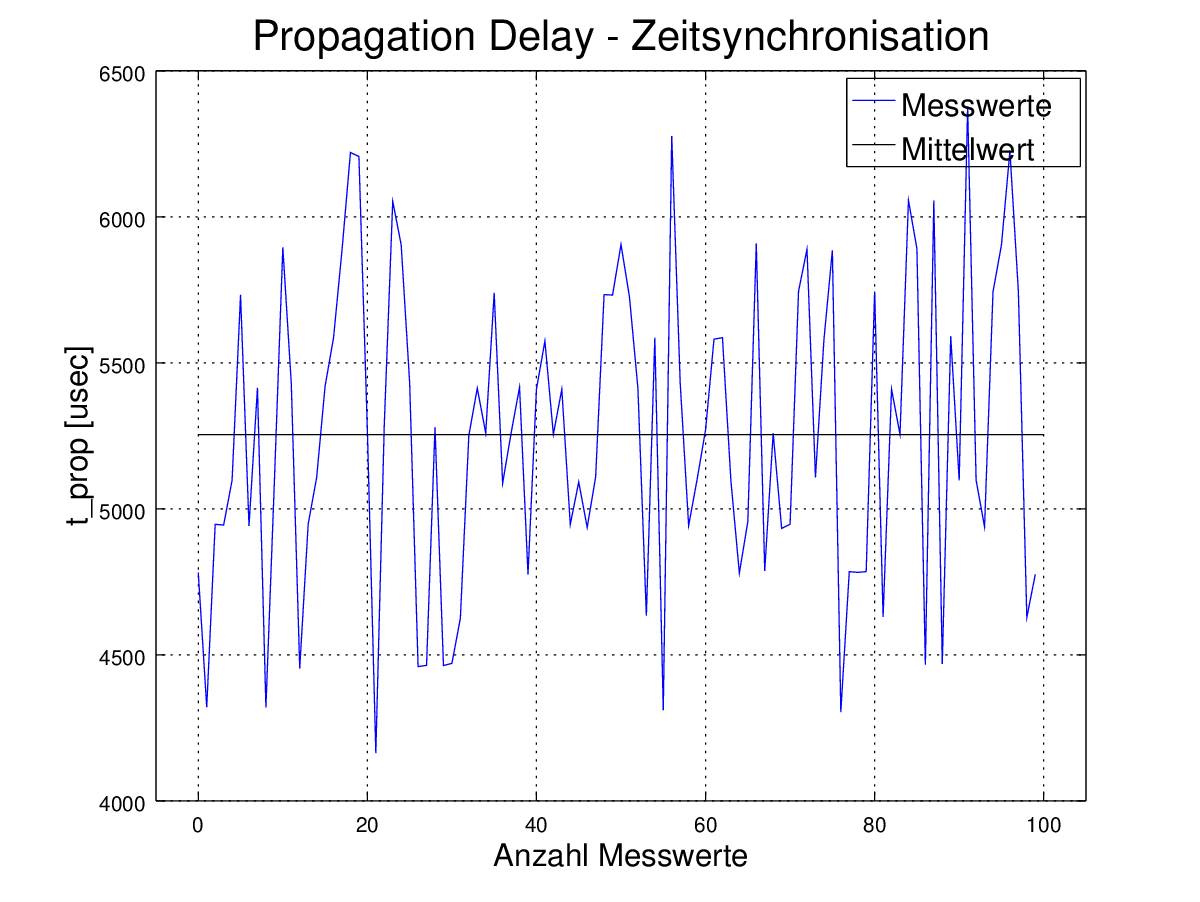
\includegraphics[width=1.2\textwidth]{images/t_prop_zeit_sync_figure.png}
        \caption{Messwerte von $t_{prop}$ bei hundert Messungen}
        \label{img:zeit_sync_t_prop_figure}
\end{figure}

Die obige Abbildung \ref{img:zeit_sync_t_prop_figure} zeigt die Laufzeitverzögerung bei \si{100} Messungen. Da die Messwerte sich im Millisekundenbereich bewegen, bedeutet dies für die Zeitsynchronisation falsche Ergebnisse. PTP verlangt für Zeitsynchronisation gleiche Laufzeitverzögerungen. Da diese im Millisekundenbereich schwanken, ist es zu erheblichen Abweichungen bei der Synchronisation gekommen. Neben der Laufzeitverzögerung spielt noch das Hinzufügen der Systemzeit in das Paket eine Rolle. Je später die Systemzeit in das UDP-Paket eingefügt wird, desto weniger Fehler gibt es bei der Zeitsynchronisation. Bei PTP muss die Systemzeit genau dem Aussenden entsprechen; deswegen ist die Systemzeit so spät wie möglich zum Paket hinzuzufügen. Passiert dies nicht, geht Genauigkeit verloren, weil das Zusammenbauen des UDP-Pakets Zeit kostet. Eine Vermutung für die Abweichungen bei der Laufzeitverzögerung ist, dass die Funktion $udp\_receive\_packet()$ durch Polling abgefragt wird. Somit gehen Pakete verloren und werden nur zu einem bestimmten Zeitpunkt entgegengenommen. RIOT bietet keine Interruptroutine für das Empfangen von Paketen an. Somit können Pakete verloren gehen, welches sich kritisch auf die Zeitsynchronisation auswirkt. Weiterhin ist eine kleine Abweichung von Master und Slave nicht zu verhindern. Da jeder Frequenzgeber schwingt, kommt nicht jeder Taktpegel exakt genau an. Der Jitter gibt an, um wieviele Nanosekunden der Frequenzgeber abweichen kann. Dieser ist beim Master und Slave minimal unterschiedlich.

\subsection{\funkempfaenger}
Um die Abweichung der Zeitsynchronisation aufzufangen, wird der \funkempfaenger \platz für das Startsignal einer Messung verwendet. Dafür muss allerdings der Empfänger ein eindeutiges Signal erhalten. Dies ist ein \si{LOW}-Signal. Da eine solche Abweichung für eine zentimetergenaue Positionsbestimmung nicht vertretbar ist, wird für den Start der Messung ein \funkempfaenger \platz verwendet. Für den Testaufbau wurde der Empfänger an das Oszilloskop angeschlossen. Der \si{DATA}-Eingang des Senders wurde mit dem \board \platz verbunden. Das Board produziert eine \SI{1}{\hertz} Frequenz auf dem verbunden Pin. Das Oszilloskop sollte nun diese Frequenz wiederspiegeln. Das Messergebnis ist in Abbildung \ref{img:ausgang_sender_pin} dargestellt. Es ist zu erkennen, dass das Mikrofon ein Rauschen erkennt. Dies belegen die vielen kurzen \si{LOW}-Pegel. Als vom Sender ein \si{LOW}-Pegel übertragen wurde, konnte nicht eindeutig bestimmt werden, ob das Signal angekommen war oder durch das Rauschen unterging. Die Pegelwechsel A-E belegen, dass sich kein Pegelwechsel am Ausgang eindeutig vom Rauschen abhebt. Somit kann diese Variante nicht als Startsignal verwendet werden. Der Funkempfänger scheidet damit aus.

\begin{figure}[H]
        \centering
        \hspace*{-1.7cm}
        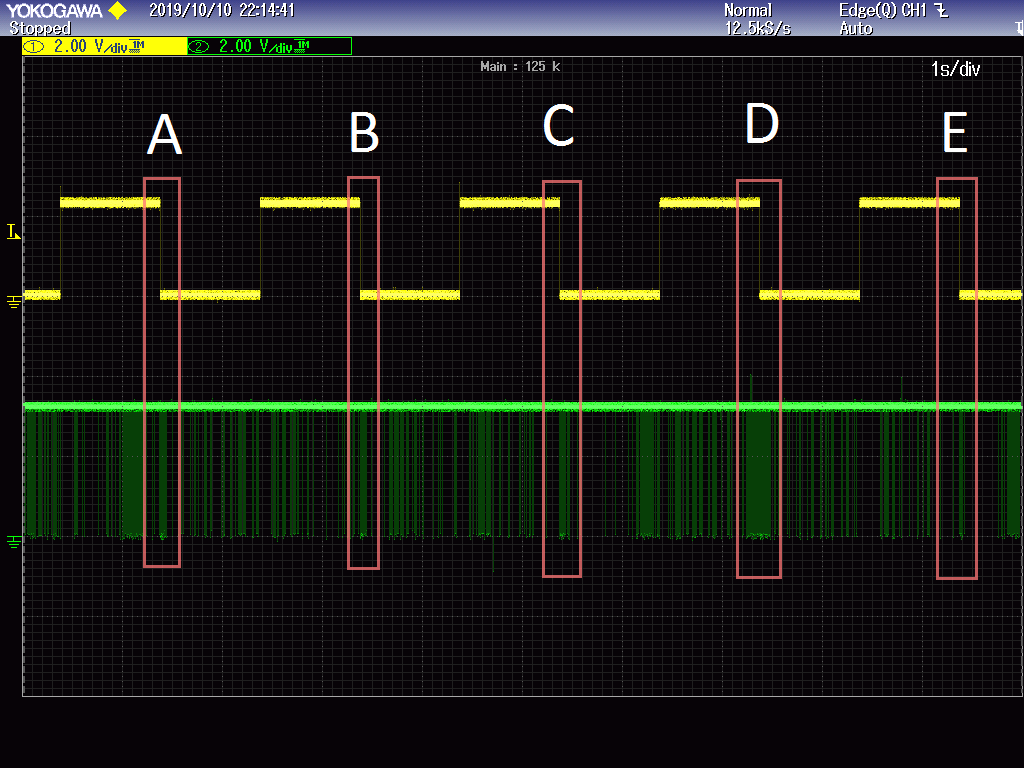
\includegraphics[width=1.2\textwidth]{images/schmitt_trigger_billig_sender_bearbeitet.png}
        \caption{\si{DATA}-Pin des \funkempfaenger \platz Empfänger}    
        \label{img:ausgang_sender_pin}
\end{figure}

\subsection{Software}
Für die Positionsbestimmung verhält sich die Software nach dem Programmablaufplan - siehe Abbildung \ref{img:PAP}. Zuerst wird der Zeitunterschied ausgeglichen, der zwischen dem Master und dem Slave besteht. Dafür wird das bereits beschriebene PTP Protokoll verwendet. Erst nachdem die Zeitsynchronisation erfolgreich ist, werden Messungen vorgenommen. Dabei spricht der Master einzeln die Slaves an. Der Master gibt zu einem bestimmten Zeitpunkt vor, wann der entsprechende Slave den Lautsprecher für \SI{40000}{\mu\s} einschaltet. Über das Mikrofon beim Master wird der Ton empfangen und sofort die Systemzeit bestimmt. Über die Differenz vom Aussenden und Empfangen kann die Distanz berechnet werden.
\begin{figure}[H]
        \centering
        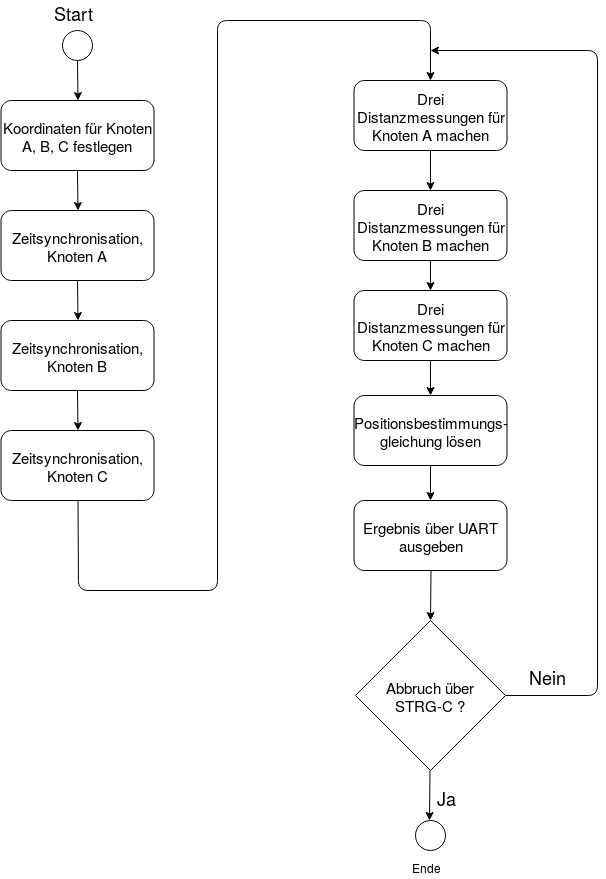
\includegraphics[width=0.8\textwidth]{images/PAP.png}
        \caption{Programmablaufplan der Software}
        \label{img:PAP}
\end{figure}

Dieses Vorgehen wird für alle drei Slaves wiederholt. Zusammen mit den Koordinaten der Slaves ergeben sich auf einer Ebene drei Kreise, die sich schneiden. Der Schnittpunkt der Kreise ist foglich die Position des Masters. Dabei ist zu beachten, dass der Master sich während der drei Messungen nicht bewegen darf - sonst werden die Ergebnisse verfälscht. Mit den drei Distanzen wird die Position bestimmt. Die Funktion für die Positionsbestimmung wurde von github (pepebecker/circle-intersection) entnommen \cite{src_GITHUB_CODE}. Wird die Software nicht abgebrochen, wiederholt sich die Messung für alle Slaves. Somit kann sich der Master auf der Ebene bewegen und bekommt seine Postion angezeigt. Es muss beachtet werden, dass durch den Jitter des Frequenzgebers die Systemzeit der Slaves mit der Zeit divergiert, d.h, wartet man entsprechend lange, ist die Systemzeit der Slaves nicht mehr übereinstimmend mit dem Master. Deswegen muss regelmäßig eine Zeitsynchronisation erfolgen. Da diese Arbeit unter Laborbedinungen durchgeführt wird, gibt es nur eine Zeitsynchronisation.

